\documentclass[border=10pt]{standalone}
\usepackage{amsmath,amssymb}
\usepackage{pgfplots}
\pgfplotsset{compat=1.18}
\usetikzlibrary{arrows.meta}
\usepackage{amsmath}

\begin{document}
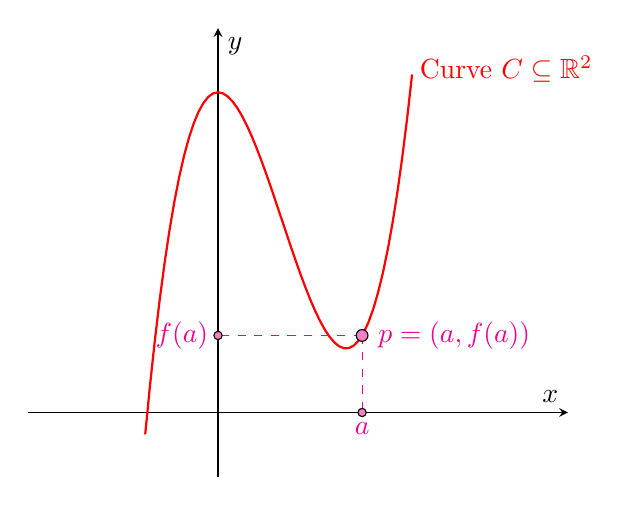
\begin{tikzpicture}
% --- Pre-calculate all values for the new function ---
% Define the function y = (x+1)(x-2)(x-2)+1 
% = (x+1)(x^2-4x+4)+1 = x^3-4x^2+4x+x^2-4x+4+1=x^3-3x^2+5
% and its derivative y' = 3x^2-6x
\pgfmathsetmacro{\a}{2.25}              % x-coordinate of point p
\pgfmathsetmacro{\ay}{\a^3-3*\a^2+5} % y-coordinate using the new function
\pgfmathsetmacro{\slope}{3*\a^2 -6*\a} % Slope using the new derivative

\pgfmathsetmacro{\dx}{1}             % Vector x-component (made slightly smaller for visibility)
\pgfmathsetmacro{\dy}{\slope * \dx}   % Vector y-component
\pgfmathsetmacro{\endx}{\a + \dx}     % Vector end-point x
\pgfmathsetmacro{\endy}{\ay + \dy}     % Vector end-point y

% --- Pre-calculate label position for the tangent line ---
\pgfmathsetmacro{\labelx}{\a + 0.5}
\pgfmathsetmacro{\labely}{\ay + \slope*(\labelx-\a)}

\begin{axis}[
axis lines=center,
xlabel=$x$, ylabel=$y$,
xtick=\empty,ytick=\empty,
legend pos=north west,
xmin=-2.5, xmax=5,   % Adjusted axis limits
ymin=-1, ymax=6,    % Adjusted axis limits
restrict y to domain=-1:6,
axis equal, % Ensures slopes are visually correct
clip=false,
]

% --- Plot the curve y = x^3 + x^2 + 1 ---
\addplot[domain=-2.5:5, samples=100, thick, red] {(x+1)*(x-2)*(x-2) + 1};
\node[above right, red] at (axis
cs: 3, 3^3-3*3^2+5) {Curve $C\subseteq\mathbb{R}^2$};
%		\node[right] at (axis cs: 2.5+2, 2.5^3 + -3 *2.5 + 9) {Curve $C\subseteq\mathbb{R}^2$};
%\addlegendentry{curve $C\subseteq\mathbb{R}^2$};

% --- Plot the tangent line at x=a ---
%		\addplot[domain=-1:3.5, samples=2, blue] {\ay + \slope*(x-\a)};
%		\node[right, blue] at (axis cs:3.5, 3*3^2-13) {$y=f'(x)$};
%		\node[right] at (axis cs: 3.5+2, 3*3^2-13) {Tangent Space $T_pC$};
%\node[right, rotate=atan(\slope), black!60] at (axis cs: \labelx, \labely) {$T_pC$};

%		% --- Draw the tangent vector v ---
%		\draw[
%		-{Stealth},
%		thick,
%		cyan,
%		] (axis cs: \a, \ay) -- (axis cs: \endx, \endy)
%		node[right] {$\mathbf{v} = \langle 1, f'(a) \rangle$};
%		%node[midway, above, sloped] {$v = \langle dx, (3a^2+2a)dx \rangle$};
%		\draw[dashed, cyan] (\a,\ay) -- (\a+1,\ay) node[midway,below] {$1$};
%		\draw[dashed, cyan] (\a+1,\ay) -- (\a+1,\ay+\slope) node[midway,right] {$f'(a)$};
%		
%		
% --- Mark the point p ---
\draw[dashed, magenta] (\a,\ay) to (\a,0) node[below] {$a$};
\draw[dashed, magenta] (\a,\ay) to (0,\ay) node[left] {$f(a)$};
\node[circle, fill=magenta!50, draw=black, inner sep=1.5pt, label={right:$\color{magenta}p=(a,f(a))$}] at (axis cs: \a, \ay) {};

\draw[fill=magenta!50] (\a,0) circle (1.5pt);
\draw[fill=magenta!50] (0,\ay) circle (1.5pt);
%		\foreach \x in {-.5}
%			\addplot[domain=-2:2, samples=7, green] {(\x)^3 - 3*(\x) + 9) + (3*(\x)^2 -3)*(x-(\x))};

\end{axis}
\end{tikzpicture}
\end{document}